% Rapport final Dream in Orbit, 16 novembre 2026. Compilation : tectonic rapport_final_2026.tex (ou xelatex).
% Figures : figures_final.py (voir l'annexe) ; démo : ../demo/reve_contre_realite.png (outils/demo.py).
\documentclass[11pt,a4paper]{article}

\usepackage{fontspec}
\usepackage{unicode-math}
\setmainfont{texgyreschola}[Extension=.otf, UprightFont=*-regular, BoldFont=*-bold,
  ItalicFont=*-italic, BoldItalicFont=*-bolditalic]
\setmathfont{texgyreschola-math.otf}
\setmonofont{texgyrecursor}[Extension=.otf, UprightFont=*-regular, BoldFont=*-bold, Scale=0.9]
\usepackage{polyglossia}
\setmainlanguage{french}

\usepackage[a4paper,margin=2.3cm,top=2.2cm,bottom=2.4cm]{geometry}
\usepackage{microtype}
\usepackage{graphicx}
\usepackage{booktabs}
\usepackage{tabularx}
\usepackage{array}
\usepackage[table]{xcolor}
\usepackage{caption}
\usepackage{float}
\usepackage{enumitem}
\usepackage{tikz}
\usetikzlibrary{positioning,arrows.meta,fit,calc}
\usepackage{fancyhdr}
\usepackage[hidelinks]{hyperref}

\definecolor{bleu}{HTML}{2A78D6}
\definecolor{orange}{HTML}{EB6834}
\definecolor{violet}{HTML}{8A5CC2}
\definecolor{encre2}{HTML}{52514E}
\definecolor{fond}{HTML}{F3F2EE}
\definecolor{trait}{HTML}{9A9890}

\captionsetup{font=small,labelfont=bf,labelsep=period,justification=justified,singlelinecheck=false}
\setlist{itemsep=2pt,topsep=4pt}
\setlength{\parskip}{4pt}
\renewcommand{\arraystretch}{1.12}
\newcommand{\code}[1]{\texttt{#1}}
\setlength{\emergencystretch}{2em}
\newcolumntype{R}{>{\raggedleft\arraybackslash}X}

\pagestyle{fancy}
\fancyhf{}
\fancyhead[L]{\small\color{encre2}Dream in Orbit, rapport final}
\fancyhead[R]{\small\color{encre2}16 novembre 2026}
\fancyfoot[C]{\small\color{encre2}\thepage}
\renewcommand{\headrulewidth}{0.4pt}

\begin{document}

\thispagestyle{plain}
\begin{center}
  {\LARGE\bfseries Dream in Orbit}\\[4pt]
  {\large Rapport final : world model de la consommation électrique d'un satellite}\\[8pt]
  {\color{encre2}Max DENIS \quad·\quad 16 novembre 2026 \quad·\quad branche \code{main}, commit \code{c3b4dc8}}
\end{center}

\vspace{4pt}
\noindent\colorbox{fond}{\parbox{\dimexpr\linewidth-2\fboxsep}{\small
\textbf{En bref.} Le modèle livré (structure S2) mélange à parts égales une part réseau et une part boosting. La part réseau contient deux world models GRU de natures différentes : un GRU qui avance sur le seul contexte et un GRU qui relit sa propre prédiction à chaque heure. La part boosting corrige heure par heure, sans mémoire. Trois circuits ont un traitement spécialisé. Le modèle obtient une RMSE de 0.0746 en validation directe (entraînement sur annee1, simulation de annee2) et de 0.0805 en validation inverse, soit 0.0775 en moyenne. La prédiction constante fait 0.1155, le meilleur boosting seul du début du projet 0.0975, le premier world model complet 0.0897. Le gain sur la constante est de 33 \%. Sur quatre coupures glissantes avec réentraînement, la moyenne vaut 0.0737. S2 n'est pas le meilleur score interne mesuré (0.0763 pour la structure C1) : c'est un choix de sobriété, expliqué en section~\ref{sec:sobriete}.}}

\vspace{6pt}
Ce rapport fait suite aux rapports d'avancement du 4 et du 8 novembre, qui détaillent les premières étapes. La partie~I retrace le chemin suivi, du premier essai au modèle livré, avec ce qui a été gardé, rejeté et pourquoi. La partie~II décrit le modèle final et ses résultats : architecture, scores, dérive, démo « rêve contre réalité », erreurs, incertitude et ablations. Les scores sont des RMSE calculées par \code{evaluate.py}, avec un point décimal.

%=====================================================================
\part*{Partie I \quad Le processus}
\addcontentsline{toc}{part}{Partie I : le processus}

\section{Données et protocole}

\subsection{Fiche des données}

Le kit contient deux périodes consécutives de télémétrie réelle de 687 jours chacune (16\,488 heures) : annee1 du 22/08/2008 au 09/07/2010, annee2 du 10/07/2010 au 26/05/2012. La cible est la moyenne horaire de chacun des 33 circuits ; une heure sans mesure n'est pas notée (32 heures dans annee1, 246 dans annee2). La synthèse d'exploration (\code{docs/exploration/synthese\_exploration.pdf}) donne le détail.

\begin{table}[!htb]
\centering\small
\caption{Fichiers du kit et nombre de lignes par période.}
\label{tab:fichiers}
\begin{tabularx}{\linewidth}{l l X r r}
\toprule
Fichier & Rôle & Contenu d'une ligne & annee1 & annee2 \\
\midrule
\code{power.csv}  & état    & courant des 33 circuits, une mesure toutes les 32 s environ & 1\,830\,121 & 1\,768\,248 \\
\code{dmop.csv}   & actions & commande envoyée à un sous-système & 187\,126 & 143\,802 \\
\code{ftl.csv}    & actions & intervalle de pointage, avec ou sans communication & 19\,571 & 20\,051 \\
\code{saaf.csv}   & contexte & angles du Soleil par rapport au satellite & 1\,261\,290 & 1\,305\,759 \\
\code{evtf.csv}   & contexte & événement daté (éclipse, occultation, péricentre\ldots) & 76\,776 & 75\,208 \\
\code{ltdata.csv} & contexte & valeurs journalières (distances, durée des éclipses) & 687 & 687 \\
\bottomrule
\end{tabularx}
\end{table}

Trois constats de l'exploration ont pesé sur tout le projet.
\begin{itemize}
  \item \textbf{Amplitudes très inégales.} NPWD2451 et NPWD2551 ont des écarts-types de 0.84 et 0.61 sur annee1, d'autres circuits sont presque constants. La RMSE n'est pas pondérée : les circuits variables font le score.
  \item \textbf{Niveaux qui changent d'une période à l'autre.} NPWD2851 passe de 0.20 à 0.32 en moyenne, NPWD2531 de 0.12 à 0.01. Un modèle qui apprend le niveau d'une période se trompe d'office sur l'autre.
  \item \textbf{Cadences et recouvrements.} \code{ftl} contient 695 intervalles qui chevauchent le précédent dans annee1, \code{dmop} s'arrête 12.6 jours avant la fin de \code{power} dans annee2. Tout est ramené sur une grille horaire commune, sans compter deux fois une durée.
\end{itemize}

\subsection{Protocole de validation}

Chaque essai passe par la chaîne complète \code{train.py}, \code{predict.py}, \code{evaluate.py}, jamais par un découpage aléatoire des heures. Deux directions servent de référence : directe (annee1 \textrightarrow{} annee2) et inverse (annee2 \textrightarrow{} annee1). Le score est la moyenne des deux. La direction inverse a écarté plusieurs réglages qui ne marchaient que dans un sens.

Le protocole s'est durci au fil du projet. Au départ, un changement était gardé s'il faisait baisser la moyenne. Après la mesure du bruit de graine (environ 0.0015), il a fallu un gain d'au moins 0.0015 sans direction dégradée, ou une confirmation sur une seconde série de graines. À partir du 13 novembre, une validation chronologique a été ajoutée, puis remplacée le 15 novembre par une validation à origine glissante : quatre coupures dans annee2 (à 50, 62,5, 75 et 87,5 \% de la durée totale), avec réentraînement complet sur tout ce qui précède chaque coupure. Pour les deux dernières décisions, la liste des candidats et la règle de choix ont été écrites avant tout calcul de score.

\section{Étapes du projet}

La figure~\ref{fig:progression} résume la progression du modèle livré. Le projet se découpe en cinq phases.

\begin{figure}[!htb]
\centering
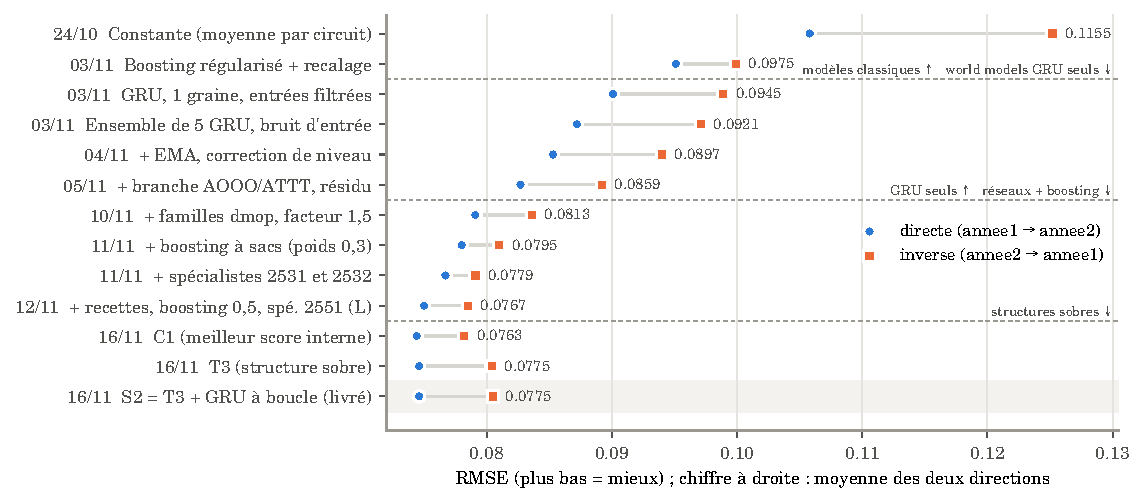
\includegraphics[width=\linewidth]{figures_final/progression.pdf}
\caption{Progression du modèle installé dans \code{poids/}, de la constante au modèle livré. Chaque ligne relie la RMSE directe (rond) et la RMSE inverse (carré) d'une configuration. Les deux dernières lignes sont moins bonnes que C1 : ce sont des choix de sobriété (section~\ref{sec:sobriete}).}
\label{fig:progression}
\end{figure}

\subsection{Phase 1 : baselines (jusqu'au 3 novembre)}

La prédiction constante (moyenne de chaque circuit sur l'entraînement) donne 0.1058 en directe et 0.1252 en inverse. Une régression Ridge heure par heure descend à 0.0994 en directe, mais elle illustre le piège des niveaux : sur annee1, NPWD2531 suit la distance au Soleil avec une corrélation de $-0.998$, et la Ridge extrapole cette relation sur annee2, où le circuit est presque éteint (0.208 contre 0.138 pour la constante).

Un gradient boosting par circuit, puis un recalage sur les 7 jours de \code{power\_init} qui s'estompe avec une demi-vie de 1440 heures, mène à 0.0951 / 0.0999. Deux leçons en sont sorties : le niveau des 7 premiers jours ne vaut que quelques semaines, et plus le modèle est contraint, mieux il passe d'une période à l'autre (100 itérations et 7 feuilles battent 600 itérations et 63 feuilles).

\subsection{Phase 2 : le world model GRU (3 au 8 novembre)}

\paragraph{Premier échec et diagnostic.} Le premier GRU faisait 0.1148 en directe, pire que le boosting, avec une erreur qui montait au fil de la période. Un réseau sans mémoire faisait encore pire (0.156) : le problème venait donc des entrées, pas de la récurrence. Dix-sept variables presque constantes sur annee1 (couverture \code{saaf}, indicateurs de valeur inconnue) avaient un écart-type minuscule ; dès qu'elles bougeaient sur annee2, leurs valeurs normalisées explosaient. Écarter ces variables et borner les entrées à leur plage d'entraînement a amené le GRU à 0.0901 / 0.0989, devant le boosting.

\paragraph{Architecture encodeur-simulateur.} Un encodeur lit les 7 jours réels et fixe l'état initial ; un simulateur GRU avance ensuite heure par heure sur le contexte seul, sans jamais relire ses sorties. Il s'entraîne sur des épisodes d'un an coupés en morceaux de 30 jours, donc sur l'horizon réel de l'évaluation. Ont été gardés : un ensemble de graines (dont l'écart-type donne l'incertitude), du bruit sur les entrées, un second membre aux variables différentes, la moyenne exponentielle des poids, puis une correction de niveau tirée de \code{power\_init} qui s'estompe avec une demi-vie apprise (0.0897 au 4 novembre).

\paragraph{Commandes et correction sur le résidu.} En regardant NPWD2881 heure par heure, j'ai vu qu'il s'allume et s'éteint avec des commandes AOOO et ATTT précises. Données au GRU comme les autres variables, elles l'aidaient en directe mais apprenaient des relations propres à annee2 sur d'autres circuits. Une petite branche qui ne nourrit que la colonne NPWD2881 a réglé le problème. La correction de niveau a ensuite porté sur le seul résidu que le contexte n'explique pas, avec un terme rapide et un terme lent (0.0859, puis 0.0854 avec une borne plus large à la prédiction).

\paragraph{Rejetés.} Les 399 variables de la version v2 complète (0.1025), l'état « dernière commande » des sous-systèmes (corrélé à 0.75 avec NPWD2551 sur annee1, faux sur annee2), un spécialiste GRU pour NPWD2551 et NPWD2451, une tête de régime partagée qui classait bien le régime mais dont la calibration changeait d'une période à l'autre. Presque tous ces rejets ont la même cause : une relation nette sur une période qui ne tient pas sur l'autre.

\subsection{Phase 3 : réseaux et boosting ensemble (10 au 12 novembre)}

Les graines d'un même GRU se trompent de la même façon : l'ensemble manquait de diversité. Un boosting à sacs temporels (cinq sacs, chacun sans un cinquième contigu de la période), enrichi de variables physiques (flux solaire par face) et de comptes par famille de commandes, a fait 0.0885 seul, presque au niveau du GRU. Mélangé au GRU avec un poids fixé d'avance par une règle écrite, il gagnait 0.0026.

Le diagnostic « d'où vient l'erreur d'une année à l'autre » a montré que le passage d'une année à l'autre n'était pas la cause principale : le GRU se trompe au moins autant hors bloc dans sa propre année. Deux causes identifiées ont été corrigées : les familles de commandes \code{dmop} (le code sans sa lettre de variante) en entrée du GRU, et un facteur 1,5 sur la correction de niveau, estimé hors bloc sur l'année d'entraînement (0.0813). Ensuite, en deux jours :
\begin{itemize}
  \item mélange 0.7 GRU + 0.3 boosting enrichi : 0.0795 ;
  \item spécialistes NPWD2531 (porte par marqueurs du planning) et NPWD2532 (boosting et GRU physique) : 0.0779 ;
  \item second GRU plus petit et plus régularisé, boosting « recette » et poids du boosting à 0.5, boosting propre à NPWD2551 : 0.0767 (modèle « L »).
\end{itemize}
Un GRU autorégressif classique (sorties réinjectées, scheduled sampling) a été essayé dans cette phase : il ne dérivait pas sur 680 jours, mais perdait 0.006 en moyenne, surtout au début de l'inverse. Il a été rejeté.

\subsection{Phase 4 : NPWD2551, la limite (13 au 15 novembre)}

NPWD2551 et NPWD2451 faisaient plus de la moitié de l'erreur. Avec ces deux circuits parfaits, la RMSE serait passée de 0.0795 à 0.0560 : le plafond était connu. Ce sont des réchauffeurs à thermostat tout-ou-rien, avec des créneaux de 5 à 20 minutes ; le courant brut de NPWD2551 est la somme de trois lignes de chauffage (0.205, 0.63, 1.045). La moyenne horaire dépend de la phase des cycles, qu'aucune entrée ne donne : 61 à 76 \% de la MSE de NPWD2551 est horaire.

Cinq programmes ont attaqué ce circuit : XGBoost diversifiés, fenêtres passées et futures jusqu'à 720 heures, commutateur de chauffage reconstruit depuis les commandes, porte asymétrique, modèle à deux régimes, recette de boosting reproduite au bit près, boosting par ligne de chauffage, grille de 10 minutes, thermostat différentiable, LightGBM, CatBoost (17 candidats sur Kaggle au dernier programme). Plusieurs gagnaient dans une ou deux validations, aucun dans toutes. Rien n'a été installé. C'est la phase la plus coûteuse pour aucun gain de score ; elle a fixé la limite du projet et les candidats sont gardés dans \code{poids\_candidats/npwd2551/}.

\subsection{Phase 5 : sobriété et structure finale (15 et 16 novembre)}
\label{sec:sobriete}

Le modèle L avait servi à plusieurs centaines de décisions sur les mêmes validations. Un écart de 0.001 était du même ordre que l'effet d'un changement d'environnement logiciel. J'ai donc changé d'objectif : une prochaine période contiendra un régime de chauffage que les deux années connues n'ont pas, et un modèle à peu d'entrées, sans corrections apprises, devrait moins s'y dégrader qu'un modèle affûté. J'acceptais de perdre jusqu'à 0.0010 de moyenne interne pour cela.

\paragraph{Ingrédients.} Un résultat de la phase 3 a rendu cette direction possible. Un petit GRU sur 165 variables tirées des seuls contextes bruts (variables « S ») était le meilleur GRU seul en directe, mais dérivait en inverse : la période orbitale, quasi constante sur annee2, se trouve à $-43$ écarts-types en annee1. Borner chaque entrée aux minimum et maximum d'entraînement a supprimé cette extrapolation (inverse 0.098 \textrightarrow{} 0.086).

\paragraph{Choix de la structure.} Cinq structures, listées avant mesure, ont été comparées sur les deux validations et sur les quatre coupures glissantes (tableau~\ref{tab:structures}). La règle écrite d'avance a désigné C1, installé. J'ai ensuite installé T3, plus sobre, bien que la règle l'ait refusé, puis S2, qui ajoute à T3 un GRU qui relit sa propre prédiction. Pour S2, la règle ne pouvait l'écarter que sur un échec technique (sortie invalide, perte de plus de 0.003, dérive manifeste) ; aucun n'est survenu.

\begin{table}[!htb]
\centering\small
\caption{Structures comparées le 16 novembre (modèle complet avec spécialistes). Moyennes des deux validations temporelles et des quatre coupures glissantes. L et C1 : moyennes de deux groupes de 5 graines ; T1, T3 et S2 : 10 graines.}
\label{tab:structures}
\begin{tabularx}{\linewidth}{l X r r r}
\toprule
Structure & Part réseau ; part boosting ; NPWD2551 & Dir./inv. & Coupures & c87 \\
\midrule
L (livré au 15/11) & 0.7 GRU mixte + 0.3 GRU recette ; boosting R ; D3L & 0.07674 & 0.07189 & 0.06800 \\
C1 & 0.5 GRU mixte + 0.5 GRU S borné ; R ; D3L & 0.07629 & 0.07249 & 0.07110 \\
T1 & GRU S borné ; R ; D3L & 0.07678 & 0.07379 & 0.07700 \\
T3 & GRU S borné ; boosting S ; recette B & 0.07753 & 0.07416 & 0.07636 \\
\rowcolor{fond} \textbf{S2 (livré)} & \textbf{0.5 GRU S borné + 0.5 GRU à boucle ; S ; B} & \textbf{0.07753} & \textbf{0.07371} & \textbf{0.07422} \\
\bottomrule
\end{tabularx}
\end{table}

Ce choix a un coût mesuré : S2 perd 0.0008 sur la moyenne directe / inverse par rapport à L et 0.0012 par rapport à C1. En échange, il n'a plus de GRU à 268 entrées, d'épisodes de 365 jours ni de correction de niveau apprise, et sa part réseau contient deux dynamiques différentes. Il est meilleur que T3 sur la moyenne des coupures ($-0.00045$), surtout sur la dernière ($-0.0021$).

\subsection{Ce que le processus m'a appris}

\begin{itemize}
  \item \textbf{Une corrélation nette sur une période n'est pas une loi.} La Ridge sur NPWD2531, l'état des sous-systèmes, les commandes exactes en entrée du GRU, la période orbitale : chaque fois, le gain d'une direction se payait dans l'autre. La validation inverse a été le meilleur détecteur.
  \item \textbf{Contraindre avant d'agrandir.} Les gains durables viennent de filtres, de bornes et de branches restreintes, rarement de réseaux plus grands ou de variables en plus.
  \item \textbf{Diagnostiquer avant d'essayer.} Le MLP sans mémoire, la comparaison hors bloc et le plafond de NPWD2551 ont chacun évité une série d'essais inutiles.
  \item \textbf{Écrire la règle avant le score.} Avec deux années seulement, la validation s'use. Fixer la liste des candidats et la règle avant le calcul a limité l'optimisme de sélection, et a rendu visibles les décisions prises pour d'autres raisons que le score.
\end{itemize}

%=====================================================================
\part*{Partie II \quad Le modèle final S2}
\addcontentsline{toc}{part}{Partie II : le modèle final}

\section{Architecture}

\begin{figure}[!htb]
\centering
\begin{tikzpicture}[
  font=\footnotesize,
  boite/.style={draw=trait, fill=white, rounded corners=2pt, align=center, inner sep=3pt},
  donnee/.style={draw=none, fill=fond, rounded corners=2pt, align=center, inner sep=3pt},
  fleche/.style={-{Stealth[length=2mm]}, draw=encre2, line width=0.6pt}]
  \node[donnee, text width=23mm] (ctx) at (0,0) {contextes bruts\\\code{dmop ftl evtf}\\\code{saaf ltdata}};
  \node[donnee, text width=23mm] (init) at (0,-2.3) {\code{power\_init}\\7 jours réels};
  \node[boite, text width=17mm] (vars) at (3.0,0) {variables S\\165 par heure};
  \node[boite, fill=bleu!8, text width=44mm] (g0) at (6.9,1.6) {\textbf{GRU S borné} (10 graines)\\entrées bornées, recalé};
  \node[boite, fill=violet!10, text width=44mm] (gb) at (6.9,0) {\textbf{GRU à boucle} (10 graines)\\relit $\hat y_{t-1}$, sans recalage};
  \node[boite, fill=orange!10, text width=44mm] (gbm) at (6.9,-1.6) {\textbf{boosting} à 5 sacs, recalé\\NPWD2551 : recette B};
  \node[boite, text width=19mm] (res) at (10.9,0.8) {part réseau\\$\tfrac12\,$G0 $+$ $\tfrac12\,$GB};
  \node[boite, text width=21mm] (mix) at (13.6,-0.4) {mélange\\$\tfrac12$ réseau\\$+\,\tfrac12$ boosting};
  \node[boite, text width=21mm] (spe) at (13.6,-2.1) {spécialistes\\2531 et 2532};
  \node[align=center, text width=34mm] (y) at (13.4,-3.4) {$\hat y_t$ : 33 circuits\\$\sigma$ : écart-type des 20 GRU};
  \draw[fleche] (ctx) -- (vars);
  \draw[fleche] (vars.east) -- ++(0.35,0) |- (g0.west);
  \draw[fleche] (vars.east) -- (gb.west);
  \draw[fleche] (vars.east) -- ++(0.35,0) |- (gbm.west);
  \draw[fleche, dashed] (init.east) -- ++(1.6,0) |- ([yshift=-1.5mm]gbm.west);
  \draw[fleche] (g0.east) -| (res.north);
  \draw[fleche] (gb.east) -| (res.south);
  \draw[fleche] (res.east) -| (mix.north);
  \draw[fleche] (gbm.east) -- (12.15,-1.6) |- (mix.west);
  \draw[fleche] (mix) -- (spe);
  \draw[fleche] (spe) -- (y);
\end{tikzpicture}
\caption{Structure S2. Les trois composants voient les mêmes 165 variables S, calculées à partir des seuls contextes bruts. Les 7 jours réels servent à recaler le GRU S borné et le boosting, et à réchauffer l'état du GRU à boucle (flèche en tirets, tracée vers un seul composant pour la lisibilité). Les spécialistes ne touchent que trois colonnes.}
\label{fig:archi}
\end{figure}

\paragraph{Variables S.} \code{dio/caracteristiques.py} construit 165 variables horaires à partir des contextes : fractions d'heure dans chaque type de pointage et de communication, ombre et pénombre, flux solaire par face (constante solaire × cosinus éclairé, nul dans l'ombre), géométrie de l'orbite et altitude, récence de chaque famille de commandes et de ses changements de variante, moyennes passées des flux. Le vocabulaire des commandes est appris sur la seule période d'entraînement. Aucune consommation n'entre dans ces variables.

\paragraph{GRU S borné (G0).} Une couche GRU de 128 unités, précédée d'une projection et suivie d'une tête à deux couches, dropout 0.3 et dropout des variables 0.2. Chaque entrée est bornée au minimum et au maximum d'entraînement puis normalisée : le réseau ne voit jamais une valeur hors de son domaine. Il simule sur le contexte seul, sans relire ses sorties. À la prédiction, sa sortie est recalée sur l'écart observé pendant les 7 jours réels, avec un poids qui s'estompe. Dix graines sont moyennées.

\paragraph{GRU à boucle (GB).} Même taille et mêmes variables, mais l'entrée de chaque heure contient aussi la consommation de l'heure précédente : la vérité au début de l'entraînement, puis sa propre prédiction avec une probabilité qui monte jusqu'à 1 (scheduled sampling jusqu'à $p = 0$). L'entraînement suit 16 flux continus en segments de 168 heures ; le premier segment de chaque flux reçoit la vérité. À la prédiction, les 7 jours réels servent seulement à réchauffer l'état, puis le modèle simule librement 680 jours. C'est le world model au sens du sujet : état, actions et contexte donnent l'état suivant, et le rêve se nourrit de lui-même.

\paragraph{Boosting à sacs.} Un \code{HistGradientBoostingRegressor} par circuit (600 itérations au plus, 15 feuilles, au moins 100 observations par feuille), dans cinq sacs temporels dont chacun exclut un cinquième contigu de la période ; la prédiction est la moyenne des sacs, recalée sur \code{power\_init}. Il n'a aucune mémoire et corrige le réseau heure par heure. Pour NPWD2551, il est remplacé par la recette B, un boosting propre à ce circuit.

\paragraph{Spécialistes.} NPWD2532 : 0.6 × boosting + 0.4 × un world model GRU à variables physiques. NPWD2531 : hors des marqueurs de régime repérés dans le planning, la sortie est remplacée par le niveau médian recalé. Les 30 autres colonnes ne dépendent que du mélange.

\paragraph{Pourquoi la moitié au boosting.} Le règlement impose un réseau de neurones comme modèle final, les modèles classiques n'étant que des composants. Le poids du boosting est donc plafonné à 0.5, même si 0.6 donnait des résultats proches (0.07757 contre 0.07753).

\begin{table}[!htb]
\centering\small
\caption{Composants du modèle livré (poids entraînés sur annee1 + annee2, \code{python train.py}).}
\label{tab:composants}
\begin{tabularx}{\linewidth}{X r r r}
\toprule
Composant & Entrées par heure & Poids sur disque & Entraînement \\
\midrule
GRU S borné, 10 graines & 165 & 2.9 Mo & 2 × 6 à 9 min (T4) \\
GRU à boucle, 10 graines & 165 + 33 & 3.0 Mo & 2 × 6 à 10 min (T4) \\
Boosting à sacs (33 circuits × 5 sacs) & 673 à 794 & 25 Mo & environ 15 min (CPU) \\
Spécialistes (recette B, GRU physique, marqueurs) & -- & 9.3 Mo & -- \\
\midrule
Total & & 40 Mo & prédiction 1 à 2 min (CPU) \\
\bottomrule
\end{tabularx}
\end{table}

%=====================================================================
\section{Résultats}

\subsection{Score global}

\begin{table}[!htb]
\centering\small
\caption{RMSE sur les deux validations (modèles entraînés sur une seule période). Les scores des modèles intermédiaires viennent des rapports et du journal.}
\label{tab:final}
\begin{tabular}{l r r r r}
\toprule
Modèle & Directe & Inverse & Moyenne & Gain vs constante \\
\midrule
Constante & 0.1058 & 0.1252 & 0.1155 & -- \\
Gradient boosting + recalage (3 nov.) & 0.0951 & 0.0999 & 0.0975 & $-15.6$ \% \\
World model GRU (4 nov.) & 0.0853 & 0.0940 & 0.0897 & $-22.3$ \% \\
World model GRU (8 nov.) & 0.0826 & 0.0885 & 0.0855 & $-26.0$ \% \\
Modèle L (15 nov.) & 0.0750 & 0.0785 & 0.0767 & $-33.6$ \% \\
\textbf{S2, modèle livré} & \textbf{0.0746} & \textbf{0.0805} & \textbf{0.0775} & $\mathbf{-32.9}$ \% \\
\bottomrule
\end{tabular}
\end{table}

Sur les quatre coupures glissantes, S2 fait 0.0649, 0.0632, 0.0925 et 0.0742 (moyenne 0.0737). La coupure à 75 \% est la plus difficile pour tous les modèles : elle couvre juin à décembre 2011, où la démo (figure~\ref{fig:reve}) montre aussi la plus grosse erreur sur NPWD2551.

La figure~\ref{fig:validations} montre ce que chaque part apporte. La part réseau est meilleure que le boosting sur les deux premières coupures, le boosting est meilleur en inverse et sur les deux dernières coupures. Leurs erreurs sont corrélées à 0.81 en directe et 0.87 en inverse : assez différentes pour que le mélange batte les deux parts en directe, en inverse et sur la première coupure ; ailleurs, il reste proche de la meilleure des deux, qu'on ne connaît pas d'avance. Les deux GRU se ressemblent plus (corrélation des erreurs de 0.90 à 0.98) ; le GRU à boucle compense surtout le GRU S borné sur la dernière coupure (0.0900 contre 0.0945).

\begin{figure}[!htb]
\centering
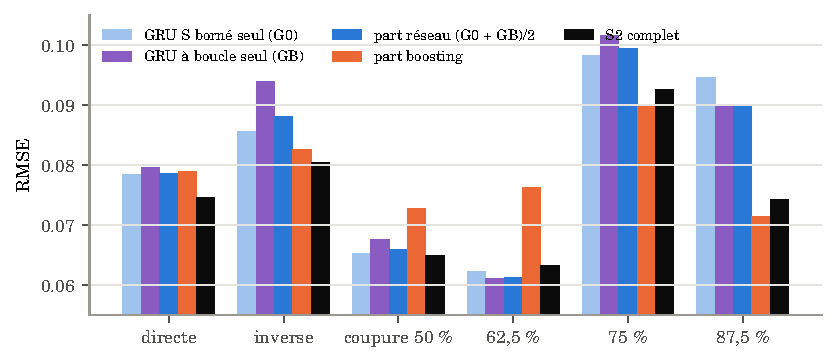
\includegraphics[width=\linewidth]{figures_final/validations.pdf}
\caption{RMSE de chaque composant et du modèle complet sur les six validations. Coupures : entraînement sur annee1 et le début d'annee2, test sur les 4\,122 heures suivantes.}
\label{fig:validations}
\end{figure}

\subsection{Dérive sur la période simulée}

\begin{figure}[!htb]
\centering
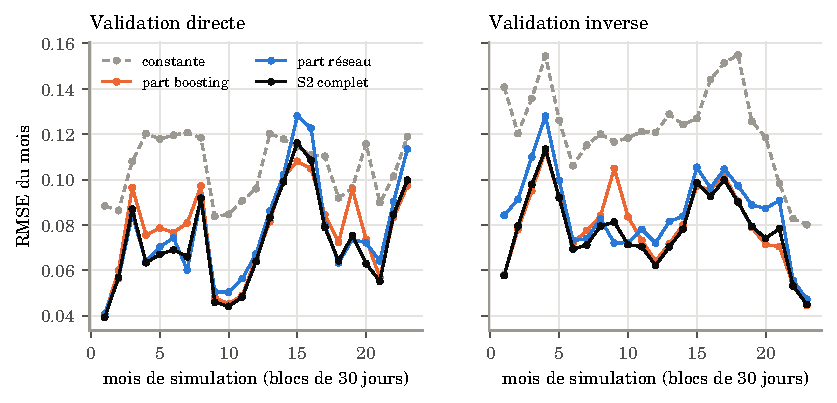
\includegraphics[width=\linewidth]{figures_final/derive.pdf}
\caption{Courbe de dérive : RMSE par bloc de 30 jours après la fin de \code{power\_init} (23 blocs, le dernier de 20 jours).}
\label{fig:derive}
\end{figure}

S2 fait mieux que la constante sur 22 blocs sur 23 en directe et sur les 23 en inverse (figure~\ref{fig:derive}). On ne voit pas de dérive qui croît avec le temps : en directe, la moyenne des cinq premiers blocs vaut 0.063 et celle des cinq derniers 0.076 ; en inverse, c'est l'inverse (0.088 puis 0.066). L'erreur suit les phases de la mission, comme celle de la constante : les pics de la directe (mois 15 et 16, octobre et novembre 2011) et de l'inverse (mois 4) touchent tous les modèles. Le GRU à boucle, qui relit sa propre sortie pendant 680 jours, ne diverge pas : le rapport entre son erreur du dernier quart et du premier quart va de 0.71 à 1.72 selon la validation, comme celui du GRU sans boucle (0.84 à 1.72).

Les deux parts se complètent dans le temps. En inverse, le boosting est nettement meilleur les quatre premiers mois (0.058 contre 0.084 le premier) : son recalage sur \code{power\_init} est plus franc. La part réseau reprend l'avantage du 9\textsuperscript{e} au 12\textsuperscript{e} mois.

\subsection{Démo : rêve contre réalité}

La figure~\ref{fig:reve} est la démo produite par \code{outils/demo.py} avec les poids de S2 entraînés sur annee1 seule. Le modèle suit bien la consommation totale et les variations lentes de NPWD2451 et NPWD2532. Sur NPWD2551, il retrouve les grandes périodes hautes (octobre 2010 à janvier 2011, juillet à novembre 2011), mais pas les coupures brusques, comme les cinq semaines à zéro de février 2011. Il surestime ce circuit d'octobre à novembre 2011, ce qui fait le pic de la courbe de dérive. Sur NPWD2851, il rate le changement de niveau de fin 2011 : le circuit monte à 0.45 et le modèle reste vers 0.28.

\begin{figure}[p]
\centering
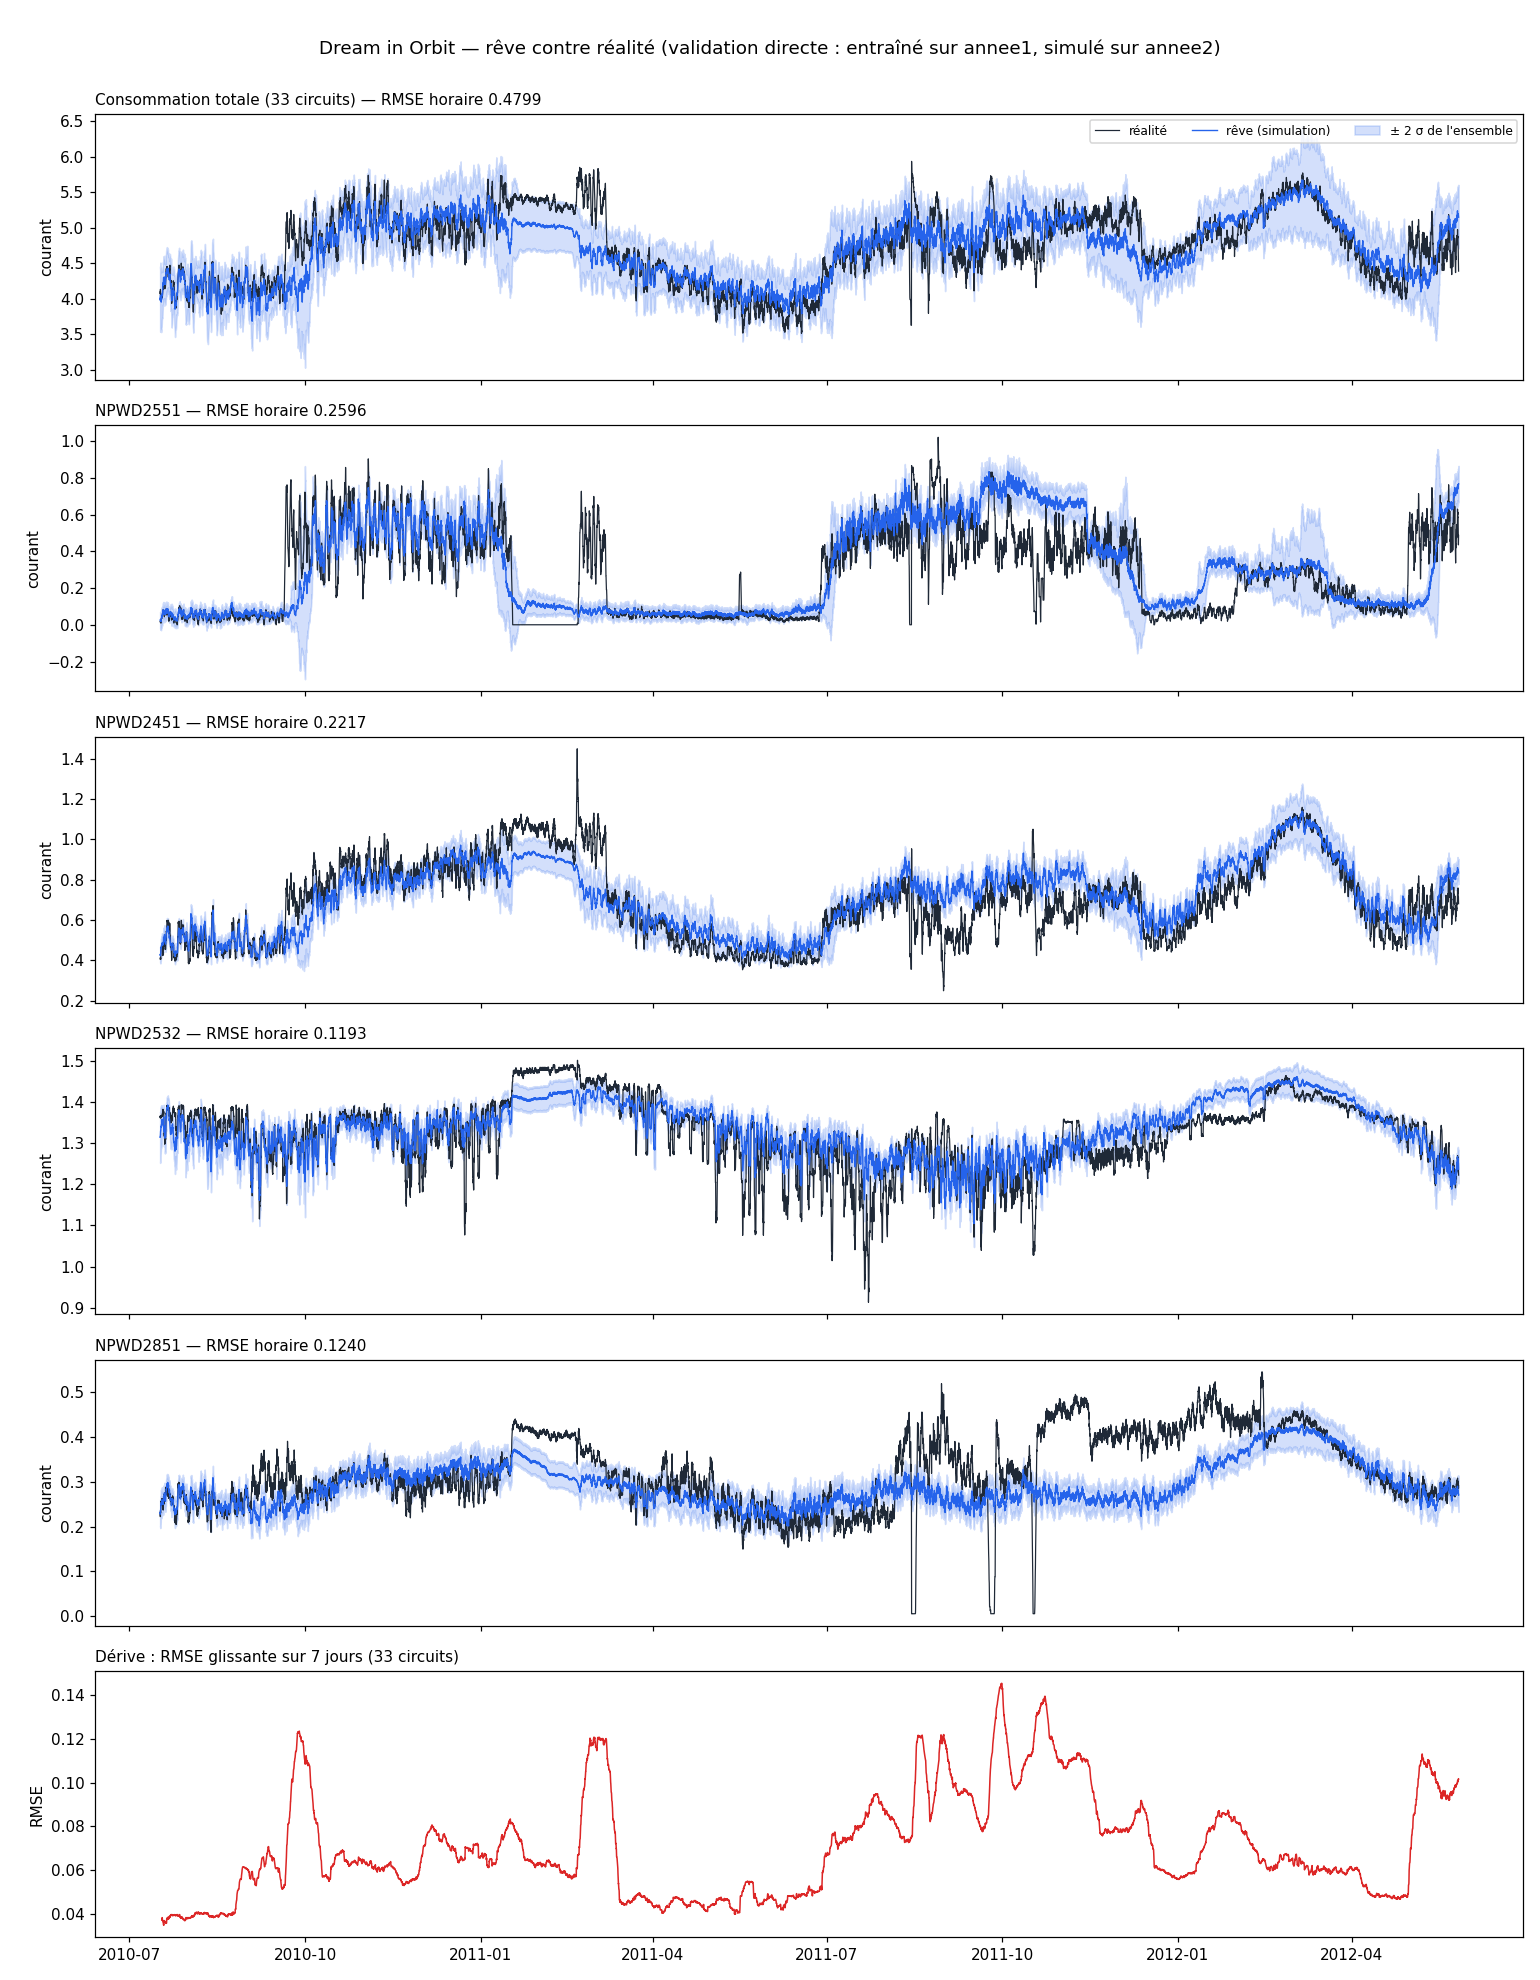
\includegraphics[width=\linewidth,height=0.86\textheight,keepaspectratio]{../demo/reve_contre_realite.png}
\caption{Rêve contre réalité sur la validation directe (entraînement sur annee1 seul, simulation de annee2 à partir de ses 7 premiers jours). Moyennes glissantes sur 24 h pour la lisibilité ; les RMSE sont horaires. La bande vaut $\pm 2$ écarts-types des 20 GRU. En bas, RMSE glissante sur 7 jours.}
\label{fig:reve}
\end{figure}

\subsection{Analyse des erreurs}

\paragraph{Par circuit.} NPWD2551 et NPWD2451 font 64 \% de l'erreur quadratique en directe et 46 \% en inverse (figure~\ref{fig:circuits}). Les huit circuits qui pèsent le plus sont tous mieux prédits que par la constante. Les deux circuits qui faisaient pire que la constante au 4 novembre sont maintenant bien en dessous : NPWD2531 passe à 0.082 en directe (constante 0.138) et NPWD2881 à 0.083 (constante 0.124). En inverse, NPWD2532 et NPWD2531 restent lourds (16 \% et 14 \%) : leur niveau change entre les périodes.

\begin{figure}[!htb]
\centering
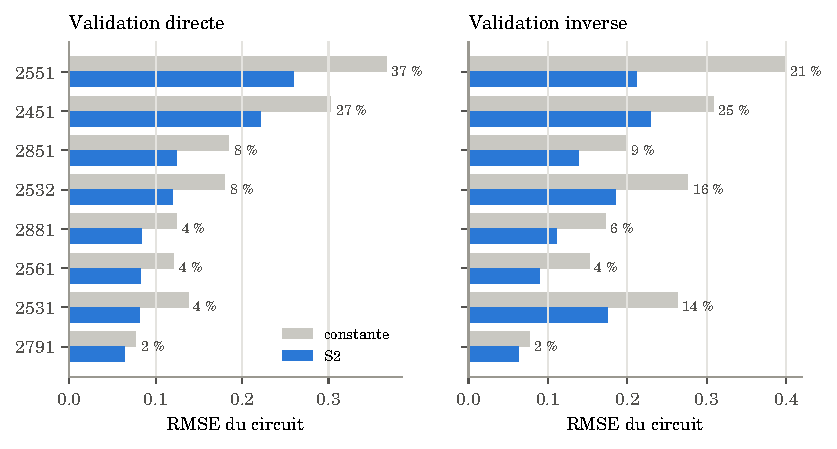
\includegraphics[width=\linewidth]{figures_final/circuits.pdf}
\caption{RMSE par circuit pour les huit circuits qui contribuent le plus à l'erreur en directe (préfixe NPWD omis). À droite des barres : part du circuit dans l'erreur quadratique de S2.}
\label{fig:circuits}
\end{figure}

\paragraph{Par échelle de temps.} J'ai découpé l'erreur de S2 en quatre bandes par moyennes glissantes : biais constant, variations lentes (plus de 30 jours), moyennes (1 à 30 jours) et rapides (moins d'un jour). La bande rapide fait 72 \% de la MSE en directe et 61 \% en inverse ; le biais constant moins de 4 \%. Les variations lentes pèsent deux fois plus en inverse (29 \% contre 14 \%), ce qui correspond aux changements de niveau entre périodes.

\paragraph{Ce qui reste hors d'atteinte.} La figure~\ref{fig:zoom} montre cinq jours de NPWD2551 et NPWD2451 heure par heure. Le modèle trouve le rythme orbital : les heures d'éclipse et de chauffage tombent au bon endroit. Mais la moyenne horaire réelle saute entre 0 et 1.2 selon la phase des cycles du thermostat, que rien dans les entrées ne donne. Le modèle prédit alors une valeur moyenne, ce qui est le meilleur choix sous une perte quadratique. Cette part de l'erreur est l'essentiel de la bande rapide.

\begin{figure}[!htb]
\centering
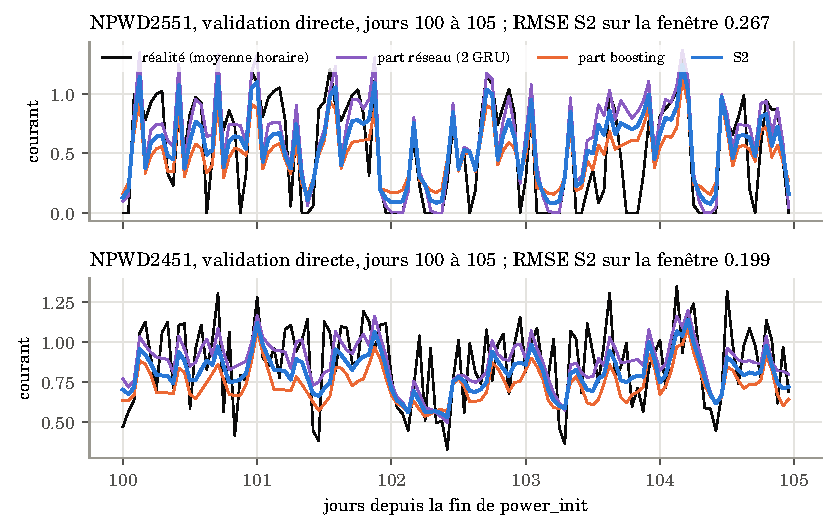
\includegraphics[width=\linewidth]{figures_final/zoom.pdf}
\caption{Cinq jours de la validation directe, valeurs horaires. La part réseau suit mieux les pointes, la part boosting les creux ; le mélange se place entre les deux.}
\label{fig:zoom}
\end{figure}

\subsection{Incertitude}

L'incertitude est l'écart-type des 20 GRU de la part réseau. Elle est trop étroite : 42 \% des valeurs réelles tombent dans la bande de $\pm 2$ écarts-types en directe et 60 \% en inverse (28 \% et 42 \% à $\pm 1$), loin des 95 \% d'une loi normale. Au 8 novembre, l'ensemble de GRU couvrait 77 à 79 \%. Trois raisons à cette baisse : les GRU sont plus petits et plus régularisés, donc plus d'accord entre eux ; l'écart-type ignore le boosting, qui fait la moitié de la prédiction ; et l'essentiel de l'erreur vient du thermostat, qu'aucun membre de l'ensemble ne voit. La bande sert à repérer les périodes où les modèles divergent (fin 2011 sur NPWD2551, par exemple), pas comme un intervalle de confiance.

%=====================================================================
\section{Ablations}

\paragraph{Structure.} Chaque ligne du tableau~\ref{tab:abl_structure} retire un élément de S2, sans réentraîner les autres. Toutes les mesures viennent du même bilan (\code{runs/gb\_bilan}).

\begin{table}[!htb]
\centering\small
\caption{Ablations de structure. Écart : différence avec S2 sur la moyenne des coupures glissantes ; positif = l'élément retiré aidait.}
\label{tab:abl_structure}
\begin{tabular}{l r r r r}
\toprule
Variante & Directe & Inverse & Moy. coupures & Écart coupures \\
\midrule
\textbf{S2 complet} & \textbf{0.07457} & \textbf{0.08050} & \textbf{0.07371} & -- \\
sans GRU à boucle (S0 = T3) & 0.07460 & 0.08045 & 0.07416 & $+0.00045$ \\
sans GRU S borné (S1) & 0.07475 & 0.08094 & 0.07376 & $+0.00005$ \\
sans spécialistes & 0.07488 & 0.08256 & 0.07374 & $+0.00003$ \\
sans boosting (part réseau seule) & 0.07862 & 0.08814 & 0.07917 & $+0.00546$ \\
sans réseau (part boosting seule) & 0.07890 & 0.08259 & 0.07756 & $+0.00385$ \\
\bottomrule
\end{tabular}
\end{table}

Le mélange réseau + boosting est l'élément le plus important : retirer une part coûte 0.003 à 0.006 en moyenne directe / inverse et 0.004 à 0.005 sur la moyenne des coupures. Ce n'est pas vrai partout : sur certaines coupures, une part seule fait mieux que le mélange (le réseau sur c62, le boosting sur c75 et c87). Les spécialistes ne jouent presque pas sur les coupures (où NPWD2531 est éteint) mais valent 0.0021 en inverse, surtout par NPWD2531. Le GRU à boucle ne change rien en directe / inverse et aide sur les coupures.

\paragraph{Réglages des GRU.} Le tableau~\ref{tab:abl_gru} isole trois choix sur les GRU seuls (10 graines chacun), entre variantes qui ne diffèrent que d'un réglage.

\begin{table}[!htb]
\centering\small
\caption{Effet d'un réglage sur la RMSE d'un GRU seul ; négatif = le réglage aide. Réinjection : comparée entre GRU à entrées bornées ; normalisation (au lieu de bornée) et recalage : sur le GRU à boucle.}
\label{tab:abl_gru}
\begin{tabular}{l r r r r r r}
\toprule
Réglage & Directe & Inverse & c50 & c62 & c75 & c87 \\
\midrule
réinjection de la sortie & $+0.0010$ & $+0.0053$ & $+0.0023$ & $-0.0016$ & $+0.0024$ & $-0.0044$ \\
normalisation standard & $+0.0001$ & $-0.0048$ & $-0.0001$ & $-0.0001$ & $+0.0003$ & $+0.0006$ \\
recalage sur \code{power\_init} & $+0.0000$ & $-0.0079$ & $+0.0002$ & $-0.0003$ & $-0.0013$ & $+0.0107$ \\
\bottomrule
\end{tabular}
\end{table}

Aucun réglage n'aide partout. La réinjection perd en directe et en inverse mais gagne sur la dernière coupure ; le recalage aide beaucoup en inverse et coûte beaucoup sur la dernière coupure. C'est ce qui justifie de garder deux GRU aux choix opposés plutôt qu'un seul : le GRU S borné est recalé et sans boucle, le GRU à boucle relit sa sortie et n'est pas recalé.

\paragraph{Groupes d'entrées et mémoire.} Les ablations par groupe d'entrées ont été mesurées sur le world model du 8 novembre (membre v1, 2 graines par direction) et n'ont pas été refaites sur S2. Elles restent la meilleure mesure de ce qu'apporte chaque source d'information au world model.

\begin{table}[!htb]
\centering\small
\caption{Ablations du world model GRU du 8 novembre (\code{docs/ABLATIONS.md}).}
\label{tab:abl_entrees}
\begin{tabular}{l r r r}
\toprule
Variante & Directe & Inverse & Écart moyen vs complet \\
\midrule
complet & 0.0840 & 0.0918 & -- \\
sans éclipses & 0.0844 & 0.0910 & $-0.0002$ \\
sans branche AOOO/ATTT & 0.0857 & 0.0939 & $+0.0019$ \\
sans \code{saaf} (Soleil) & 0.0865 & 0.0950 & $+0.0028$ \\
sans \code{dmop} (commandes) & 0.0885 & 0.0944 & $+0.0035$ \\
sans mémoire (ni encodeur ni GRU) & 0.0884 & 0.1032 & $+0.0079$ \\
\bottomrule
\end{tabular}
\end{table}

La mémoire est l'élément qui compte le plus, surtout en inverse ($+0.0114$) : sans état, le modèle ne sait pas où en est le satellite au début de la période. Les commandes et le Soleil viennent ensuite. Les éclipses ne pèsent plus rien une fois la saison portée par \code{saaf} et \code{ltdata}. Sur les variables S, une ablation isolée a aussi montré le rôle ambigu de la géométrie : la période orbitale seule porte le gain en directe ($-0.0078$) et la dérive en inverse ($+0.0128$) tant que les entrées ne sont pas bornées.

%=====================================================================
\section{Limites et travail restant}

\begin{itemize}
  \item \textbf{NPWD2551 et NPWD2451} font la moitié de l'erreur. La part qui dépend de la phase du thermostat n'est pas prévisible avec ces entrées ; la part de niveau (périodes hautes hors saison d'éclipses) l'est en partie, mais aucun des candidats testés ne gagnait dans toutes les validations.
  \item \textbf{Les choix finaux ne maximisent pas la validation interne.} T3 et S2 ont été installés pour leur sobriété, contre le classement interne (S2 perd 0.0012 sur C1). Le pari est que la sobriété tiendra mieux sur une période inconnue ; il n'est pas vérifiable avant le test.
  \item \textbf{L'incertitude est sous-estimée} (42 à 60 \% de couverture à $\pm 2\sigma$). Il faudrait inclure le boosting dans la dispersion, ou apprendre des quantiles.
  \item \textbf{Validations usées.} Directe, inverse et coupures ont servi à des centaines de décisions ; les derniers gains sont du même ordre que le bruit d'environnement (0.0001 à 0.0004).
  \item \textbf{Entraînement final non validable.} Les poids livrés sont entraînés sur annee1 + annee2 ; aucune période indépendante ne permet de les noter. Un réentraînement sur un autre matériel donne des poids proches, pas identiques au bit près.
  \item \textbf{Bonus pilote non traité.} Le GRU à boucle permettrait de simuler un planning modifié (mêmes fenêtres de communication, pointages ou commandes déplacés), à condition de rester dans la plage des plannings vus à l'entraînement, puisque ses entrées sont bornées.
\end{itemize}

%=====================================================================
\appendix
\section{Reproduire les résultats}

Environnement : Python 3.13, \code{uv sync} (ou \code{pip install -r requirements.txt}). Les entraînements ont tourné sur GPU T4 Kaggle via \code{outils/lancer\_kaggle.py}.

\begin{small}
\begin{verbatim}
python train.py                                   # modèle final S2 -> poids/
python predict.py --test_dir DOSSIER --out predictions.csv
python predict.py --test_dir DOSSIER --out p.csv \
    --options '{"sortie_incertitude": "e.csv"}'     # + écart-type des 20 GRU
python outils/valider.py --nom essai              # directe + inverse
python outils/demo.py --poids runs/essai/directe     # démo rêve contre réalité
python docs/rapport/figures_final.py --ecart DOSSIER   # figures du rapport
python -m unittest discover -s tests
\end{verbatim}
\end{small}

Le journal complet des essais est dans \code{docs/RESULTATS.md} et \code{docs/journaux/} ; les poids des candidats non retenus restent dans \code{poids\_candidats/} (git ne suit que leurs \code{INDEX.md}). Assistants IA : le projet a été mené avec des assistants IA, autorisés par le sujet ; les spécifications des recettes B et S leur sont attribuées par l'auteur, et \code{docs/PROVENANCE.md} précise ce qui vient de qui.

\end{document}
